\documentclass{beamer}

%\usepackage{verbatim}
\usepackage{anyfontsize}
\usepackage{tikz}
\usepackage{media9}

\DeclareMathOperator*{\argmax}{argmax}
\DeclareMathOperator*{\argmin}{argmin}

\newcommand{\ba}{\ensuremath{\mathbf{a}}}
\newcommand{\bb}{\ensuremath{\mathbf{b}}}
\newcommand{\bx}{\ensuremath{\mathbf{x}}}
\newcommand{\bo}{\ensuremath{\mathbf{o}}}
\newcommand{\bC}{\ensuremath{\mathbf{C}}}
\newcommand{\bq}{\ensuremath{\mathbf{q}}}


\title{
    Whale Song Unit Classification
}
\subtitle{
    Using Linear Prediction Vector Quantization\\
    and Hidden Markov Modeling
}

\begin{document}

\frame {
    \titlepage
}

\frame {
    \frametitle{The Problem}

    Following Mitchell (1997), state the problem as follows:

    \begin{itemize}
        \setlength\itemsep{1em}
        \item \textbf{Task}: \\
            Classify whale song unit instances from a given vocabulary\\
            of whale song unit types

        \item \textbf{Performance measure}:\\
            Percent of instances correctly classified

        \item \textbf{Training experience}:\\
            A database of labelled whale song unit instances
    \end{itemize}
}

\begin{frame}[fragile]
    \frametitle{Whale Song Units}

    \centering
    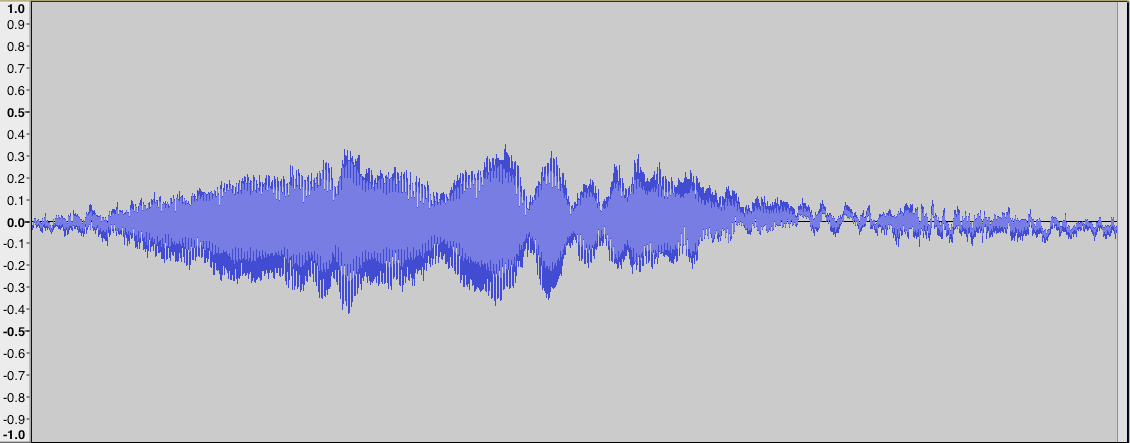
\includegraphics[width=0.7\textwidth]{from_HBSe_20151207T070326__124_45328_126_52461.png}
    \includemedia[
        height=0.44em,
        addresource=from_HBSe_20151207T070326__124.45328_126.52461.mp3,
        flashvars={
            source=from_HBSe_20151207T070326__124.45328_126.52461.mp3
            &autoPlay=true
        }
    ]{\fbox{Play}}{APlayer.swf}

    {\tiny A ``modulated cry'' instance, from \verb|HBSe_20151207T070326.wav, 124.5sec-126.5sec|}

    \begin{itemize}
        \setlength\itemsep{1em}
        \item
            Acoustic signal:
            \begin{equation*}
            \bx = \langle x_1, x_2, \ldots, x_N \rangle \qquad (N=66,283)
            \end{equation*}


    \end{itemize}
\end{frame}


\frame {
    \frametitle{Statistical Pattern Classification}

    \begin{itemize}
        \setlength\itemsep{1em}
        \item Vocabulary of $R$ song unit types:\\
            \begin{equation*}
                W = \{ w_1, \ldots, w_R \}
            \end{equation*}

        \item Assume we have a {\it model} $h_r$ for each unit type $w_r$.\\
            We are interested in computing:
            \begin{equation*}
                P[h_r|\bx] \equiv \text{Probability of $h_r$ given \bx}
            \end{equation*}

        \item Classification of an observation sequence \bx\\
            is based on a {\it maximum likelihood} model selection:
            \begin{equation*}
             h^* \equiv \argmax\limits_{h\in H} P[h|\bx]
            \end{equation*}
        where $H = \{ h_1, \ldots, h_R \}$.

    \end{itemize}
}

\frame{
    \frametitle{Maximum Likelihood model selection}

    \begin{equation*}
        \arraycolsep=1.4pt\def\arraystretch{2.2}
        \begin{array}{rcll}
            h^* &\equiv& \argmax\limits_{h\in H} P[h|\bx] \\
            &=& \argmax\limits_{h\in H} \frac{P[\bx|h] P[h]}{P[\bx]}  & \qquad \text{(Bayes' theorem)}\\
            &=& \argmax\limits_{h\in H} P[\bx|h] P[h]                 & \qquad \text{($P[\bx]$ is constant wrt $h$)}\\
            &=& \argmax\limits_{h\in H} P[\bx|h]                      & \qquad \text{(Assumming models are equiprobable)}\\
        \end{array}
    \end{equation*}
}

\frame{
    \frametitle{Linear Prediction Coding}

    \begin{itemize}
        \setlength\itemsep{1em}
        \item
        Acoustic signal:
        \begin{equation*}
        \bx = \langle x_1, x_2, \ldots, x_N \rangle
        \end{equation*}

        \item
        Transformed into a sequence of predictor vectors:
        \begin{equation*}
            \ba = \langle \ba_1, \ba_2, \ldots, \ba_T \rangle
        \end{equation*}

        \item
        Transformed into a sequence of symbols:
        \begin{equation*}
            \bo = \langle o_1, o_2, \ldots, o_T \rangle
        \end{equation*}
        where $o_t \in \{ 1, 2, \ldots, M \}$

    \end{itemize}

}

\frame{
\frametitle{Linear Prediction Coding}




\tikzset{every picture/.style={line width=0.75pt}} %set default line width to 0.75pt

\begin{tikzpicture}[x=0.75pt,y=0.75pt,yscale=-1,xscale=1]
    %uncomment if require: \path (0,379); %set diagram left start at 0, and has height of 379

    %Flowchart: Manual Operation [id:dp8594427845919483]
    \draw   (238.13,103) -- (225,63) -- (295,63) -- (281.88,103) -- cycle ;

    % Text Node
    \draw (272.5,146) node  [align=left] {What's this $\displaystyle F( x) =\int xdx$};


\end{tikzpicture}



}

\end{document}
